\chapter{Preliminaries}
% 0.5 Seiten

	In this chapter, we provide sufficient background needed to understand the algorithmic details and ideas discussed in Chapter \ref{chap:tree}.
	First, we take a look at linear optimization as a general concept and discuss necessary basics such as \ac{MIP}.
	Afterwards, these concepts are used to take a more detailed look into the characteristics of the Dantzig-Wolfe decomposition, which represents a major component of the decomposition solver \acs{GCG}.
	In addition, notations and basic definitions related to Graph Theory are introduced including the concept of \textit{Partition Refinement}; an algorithmic approach used as a building block in Chapters \ref{chap:tree} and \ref{chap:impl}.

	\section{Linear Optimization}
	% 2 Seiten
	
		\textit{Linear Optimization} is a mathematical optimization technique used to determine the best possible values for a set of variables in a given model, whose constraints or requirements are represented by linear relationships. The goal is typically to maximize or minimize a objective function, subject to a set of equality and/or inequality constraints. Both objective and constraints must be linear.
		
		If all variables are only allowed to take values from $\mathbb{R}^n_{\geq}$, i.e., only continuous values, then this optimization technique is referred to as \textit{Linear Programming}.
		In a standard form, a linear programming problem with variable vector $\mathbf{x} \in \mathbb{R}^n$, constraint matrix $A \in \mathbb{R}^{m \times n}$, objective coefficients $c \in \mathbb{R}^n$ and right-hand side vector of the constraints $b \in \mathbb{R}^m$ can be expressed as follows:
		%
		\begin{alignat}{3}
			&z^*_{LP} \; &={}	\min	&\quad  c^T && \mathbf{x} \label{eq:prelims:linprog:obj} \\
			&				  		& \text{s.t.} & \quad A && \mathbf{x} \geq b \label{eq:prelims:linprog:A} \\
			&						&					 &					&& \mathbf{x} \geq 0 \label{eq:prelims:linprog:nonneg}
		\end{alignat}
		%
		
		\clearpage
		
		\begin{figure}[ht!]
			\centering
			\begin{minipage}{0.45\textwidth}
				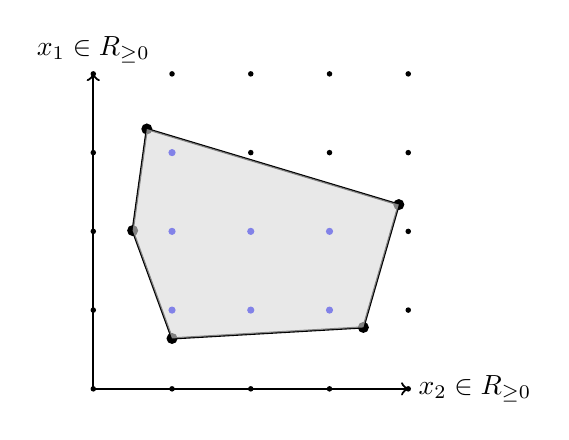
\begin{tikzpicture}[scale=1.0]
					% Grid
					\draw[->,thick] (0,0)--(4,0) node[right]{$x_2 \in \mathbb{R}_{\geq 0}$};
					\draw[->,thick] (0,0)--(0,4) node[above]{$x_1 \in \mathbb{R}_{\geq 0}$};
					
					% Beschriftung der Nebenbedingungen
					\draw[thick] (1,0.64)--(3.43,0.78);
					\draw[thick] (3.43,0.78)--(3.88,2.34);
					\draw[thick] (3.88,2.34)--(0.68,3.3);
					\draw[thick] (0.68,3.3)--(0.5,2.01);
					\draw[thick] (0.5,2.01)--(1,0.64);
					
					% Draw Points
					\fill (1,0.64) circle (2pt);
					\fill (3.43,0.78) circle (2pt);
					\fill (3.88,2.34) circle (2pt);
					\fill (0.68,3.3) circle (2pt);
					\fill (0.5,2.01) circle (2pt);
					
					\foreach \x in {0, 1, 2,3,4} {
						\foreach \y in {0, 1, 2,3,4} {
							\fill (\x, \y) circle (1pt);
						}
					}
					
					\fill[blue] (1,1) circle (1.3pt);
					\fill[blue] (2,1) circle (1.3pt);
					\fill[blue] (3,1) circle (1.3pt);
					\fill[blue] (1,2) circle (1.3pt);
					\fill[blue] (2,2) circle (1.3pt);
					\fill[blue] (3,2) circle (1.3pt);
					\fill[blue] (1,3) circle (1.3pt);
					
					% Zulässiger Bereich (grau hinterlegt)
					\fill[gray!30,opacity=0.6] 
					(1,0.64) 
					-- (3.43,0.78) 
					-- (3.88,2.34) 
					-- (0.68,3.3) 
					-- (0.5,2.01)
					-- cycle;
					
					% Drei rechtwinklige Striche am Ende
					%\foreach \i in {-0.2, 0, 0.2} {
						%	\draw[thick] 
						%	($ (3,0) + (\i,0) $) -- 
						%	($ (3,0) + (\i,0) + (45:0.2) $); % 45° ist senkrecht zur Linie (315° Linie)
						%}
				\end{tikzpicture}
			\end{minipage}%
			\begin{minipage}{0.45\textwidth}
				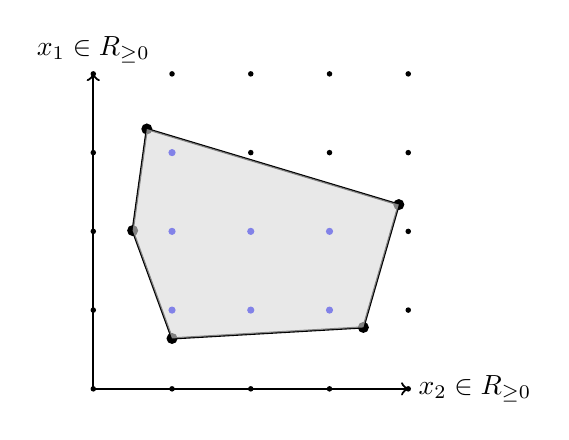
\begin{tikzpicture}[scale=1.0]
					% Grid
					\draw[->,thick] (0,0)--(4,0) node[right]{$x_2 \in \mathbb{R}_{\geq 0}$};
					\draw[->,thick] (0,0)--(0,4) node[above]{$x_1 \in \mathbb{R}_{\geq 0}$};
					
					% Beschriftung der Nebenbedingungen
					\draw[thick] (1,0.64)--(3.43,0.78);
					\draw[thick] (3.43,0.78)--(3.88,2.34);
					\draw[thick] (3.88,2.34)--(0.68,3.3);
					\draw[thick] (0.68,3.3)--(0.5,2.01);
					\draw[thick] (0.5,2.01)--(1,0.64);
					
					% Draw Points
					\fill (1,0.64) circle (2pt);
					\fill (3.43,0.78) circle (2pt);
					\fill (3.88,2.34) circle (2pt);
					\fill (0.68,3.3) circle (2pt);
					\fill (0.5,2.01) circle (2pt);
					
					\foreach \x in {0, 1, 2,3,4} {
						\foreach \y in {0, 1, 2,3,4} {
							\fill (\x, \y) circle (1pt);
						}
					}
					
					\fill[blue] (1,1) circle (1.3pt);
					\fill[blue] (2,1) circle (1.3pt);
					\fill[blue] (3,1) circle (1.3pt);
					\fill[blue] (1,2) circle (1.3pt);
					\fill[blue] (2,2) circle (1.3pt);
					\fill[blue] (3,2) circle (1.3pt);
					\fill[blue] (1,3) circle (1.3pt);
					
					% Zulässiger Bereich (grau hinterlegt)
					\fill[gray!30,opacity=0.6] 
					(1,0.64) 
					-- (3.43,0.78) 
					-- (3.88,2.34) 
					-- (0.68,3.3) 
					-- (0.5,2.01)
					-- cycle;
					
					% Drei rechtwinklige Striche am Ende
					%\foreach \i in {-0.2, 0, 0.2} {
						%	\draw[thick] 
						%	($ (3,0) + (\i,0) $) -- 
						%	($ (3,0) + (\i,0) + (45:0.2) $); % 45° ist senkrecht zur Linie (315° Linie)
						%}
				\end{tikzpicture}
			\end{minipage}
			\caption{Solution space of a linear program highlighted in gray. Point highlighted in blue represent the solution space of the corresponding integer linear program.}
			\label{fig:prelims:linear:solspace:unbounded}
		\end{figure}
		\todo{unbounded on right}
		
		Note that it is also possible to represent a set of equality $A' \mathbf{x} = b'$ by the two sets of inequalities $A' \mathbf{x} \geq b'$ and $A' \mathbf{x} \leq b'$.
		Without loss of generality, we assume optimization problems to always be minimization problems, unless explicitly stated otherwise.
		Constraints \ref{eq:prelims:linprog:A} specify a \textit{convex} polytope over which the Objective Function \ref{eq:prelims:linprog:obj} is optimized as shown in Figure \ref{fig:prelims:linear:solspace:unbounded}. A solution vector $\mathbf{x} \in \mathbb{R}_{\geq 0}$ is called \textit{feasible}, iff it satisfies both both constraints \ref{eq:prelims:linprog:A} and \ref{eq:prelims:linprog:nonneg}.
		The linear program as a whole is called \textit{feasible}, if there exists such a vector, otherwise it is considered \textit{infeasible}.
		A feasible solution $\mathbf{x} \in \mathbb{R}_{\geq 0}$ is called \textit{optimal} iff
		%
		\begin{equation*}
			c^T \mathbf{x} = \min \{ c^T \mathbf{x} \mid \mathbf{x} \; \text{is feasible} \} \iff \not\exists \mathbf{y} \in \mathbb{R}_{\geq 0}: \; \left(\mathbf{y} \; \text{feasible}\right) \land \underbrace{\left(c^T \mathbf{y} < c^T \mathbf{x}\right)}_{\mathbf{y} \; \text{is \enquote{better}}}
		\end{equation*}
		%
		If there exists a feasible solution vector, but no optimal one, then the problem is called \textit{unbounded}, as shown in Figure \ref{fig:prelims:linear:solspace:unbounded}.
		
		Linear programming is widely used in various fields such as operations research, economics, engineering, and logistics, due to its efficiency in solving large-scale real-world optimization problems. Algorithms such as the Simplex Method and Interior Point Methods are commonly used to solve LP problems efficiently.
		The simplex algorithm in particular is widely used in practice because of its efficiency on most problems, even though its worst-case complexity is exponential-time on certain families of problems depending on the chosen pivot-rule. \todo{cite}
		However, on most problems the simplex algorithm only takes a polynomial number of steps to terminate.
		For more information about how the algorithms work and their mathematical details we refer to \cite{BranchPrice}.
		
		\clearpage

		\subsection{Mixed-Integer Programs}
			%
			\begin{alignat*}{7}
				&z^*_{LP} \; &={}	\min	&\quad  c^T && \mathbf{x} && \quad+\quad && d^T && \mathbf{y} \\
				&& \text{s.t.} & \quad A && \mathbf{x} && \quad+\quad  && B && \mathbf{y} && \geq b \\
				&&&&& \mathbf{x} &&&&&& &&\in \mathbb{Q}_{\geq 0} \\
				&&&&&&&&&&& \mathbf{y} &&\in \mathbb{Z}_{\geq 0}
			\end{alignat*}
			%
			
			Even thought linear programs are already a powerful tool on its own, some problems require \textit{discrete} bounds for some variables, e.g., the $y$-variables shown in the system above. These variables are usually restricted to a subset of $\mathbb{Z}$.
			If the system contains integer \textit{and} continuous variables, then the model is called a \textit{Mixed Integer Program} (MIP).
			If only discrete variables are present, the prefix \enquote{Mixed} is omitted.
			
			MIPs are significantly more difficult to solve than pure linear programs, since the integer restrictions make the feasible region \textit{non-convex}, eliminating a key assumption of the simplex algorithm and its optimality conditions. Standard solution approaches include branch-and-bound, branch-and-cut, and cutting-plane methods, which systematically explore and prune the search space.

			It can be shown that the decision problem of whether an \acl{IP} with all variables restricted to the domain $\{ 0, 1 \}$ has a solution is NP-hard.
			Despite the higher computational complexity, MIPs are extremely powerful because they allow the modeling of a wide range of practical decision-making problems, including scheduling, routing, facility location and production planning
	
			\clearpage		
	
	\section{Dantzig-Wolfe Decomposition}
	% 3 Seiten
	
		The \textit{Dantzig-Wolfe Decomposition} is a 
		
		\clearpage
		
		Seite 2
		
		\clearpage
		
		Seite 3
	
		\clearpage
	
	\section{Graph Theory}
	% 2 Seiten
	
		Graphs are the fundamental data structure used in almost every aspect of computer science.
		This section will \textit{not} introduce new concepts not already found in standard literature about graphs and related topics.
		We will mainly introduce the notation used for the following sections and chapters.
	
		A \textit{graph} is a tuple $G = (V, E)$ with $V \subseteq \{ 1, 2, \ldots, n \}$ for some $n \in \mathbb{N}$ and $E \subseteq \{ (u, v) \mid (u, v) \in V \times V \}$. The elements of set $V$ are called \textit{vertices} or \textit{nodes}.
		The elements of set are ordered pairs called \textit{directed edges}, \textit{arcs} or simply \textit{edges} which connect two vertices with each other.
		The set of outgoing neighbors of a specific vertex $v \in V$ is denoted $E(v) = \{ (v, v') \; | \; v' \in V, vEv' \}$. 
		The set of incoming neighbors $E^{-1}(v) = \{ (v', v) \; | \; v' \in V, v'Ev \}$ is defined analogously.
		In this thesis, we will distinguish four types of graphs: directed, un-directed and bipartite, with directed being the assumed type if not stated explicitly.
		
		For \textit{un-directed} graphs, the edge relation $E$ must be symmetric $\forall u,v \in V: \; uEv \xrightarrow{} vEu$, i.e., if vertex $u$ is connected to $v$ or vice versa, then the corresponding back-edge must exists as well.
		
		\textit{Bi-partite} graphs are a special kind of graph class, where the set $V$ can be represented with two sets $L, R \subseteq V$ such that $L \cap R = \emptyset$ and $E \subseteq \{ (u, v) \mid u \in L, v \in R \}$.
		More informally, the vertex $V$ can be split into two disjoint subsets $L, R \subseteq V$ such that no edges exists between vertices in each corresponding set.
		Bi-partite graphs are especially interesting, because the relationship between variables and the constraints they participate in can be encoded as such a graph as shown in Figure \ref{fig:prelims:graphs:binpackbipartite}. This concept will be used in Chapter \ref{chap:gcg} to algorithmically detect various underlying structures. \todo{Wording}
	%
	%	A graph is called a \textit{tree} iff all unordered pairs of vertices $\{ u, v \} \in V \times V$ by \textit{at most} one path in the underlying un-directed graph.
	%
		\begin{figure}[ht!]
			\centering
			\begin{minipage}{0.47\textwidth}
				\includesvg[scale=0.9]{Bilder/DrawIO/bipart_binpack}
			\end{minipage}
			%
			\begin{minipage}{0.47\textwidth}
				\begin{align}
					&\min &\sum_{j=1}^m y_j \nonumber \\
					&\text{s.t.} &x_{11} &= 1 & \text{\textcolor{blue}{itemPacked}}_1 \nonumber \\
					&& x_{21} &= 1 & \text{\textcolor{blue}{itemPacked}}_2\nonumber \\
					&& 100 x_{11} + 99 x_{21} &\leq 200 y_1 & \text{\textcolor{blue}{binCapacity}}_1\nonumber \\
					&& x_{11}, x_{21} &\in { 0, 1 }  \nonumber \\
					&& y_1 &\in { 0, 1 } \nonumber
				\end{align}
			\end{minipage}
			\caption{A simple binpacking problem with $2$ items and $1$ bin represented as  graph.}
			\label{fig:prelims:graphs:binpackbipartite}
		\end{figure}
	
		\clearpage
	
	\section{Partition Refinement}
	\label{chap:prelims:partitionref}
	% 2 Seiten
		Partition refinement is a fundamental concept in computer science, particularly relevant in fields such as automata theory \cite{hopcroftLogALGORITHMMINIMIZING1971a}, graph theory, and model checking \cite{baierPrinciplesModelChecking2008}.
		A \textit{partition} refers to a decomposition of a finite set $U$ into disjoint, non-empty subsets $\{ A_1, A_2, \ldots, A_k \}$, called \textit{cells} or \textit{blocks}, such that:
		%
		\begin{equation*}
			\bigcup^k_{i=0} A_i = U \; \mathrm{and} \; \forall i \neq j: A_i \cap A_j = \emptyset
		\end{equation*}
		%
		The set of all partitions over a set $U$ is denoted $\Pi(U)$. A partition $\pi = \{ A_1, A_2, \ldots, A_k \}$ of a set $U$ is called a refinement of another partition $\pi' = \{ B_1, B_2, \ldots, B_m \}$, denoted $\pi \sqsubseteq \pi'$, iff
		%
		\begin{equation*}
			\forall A_i \in \pi \;\; \exists B_j \in \pi' : A_i \subseteq B_j
		\end{equation*} 
		%
		As a special case, a partition is a refinement of itself.
		More informally, partition $\pi'$ must reflect a \enquote{finer} classification of the elements than in $\pi$. 
		
		Partition refinement refers to an \textit{iterative} process that refines a given initial partition of a set over the course of multiple iterations.
		In the following, let $f: P \times Q \mapsto \Pi(A)$ be a function, which partitions the elements from $P \subseteq U$ with respect to the elements in $Q \subseteq U$. The arguments $P$ and $Q$ are called \textit{target cell} and \textit{inducing cell} respectively.
		A partition $\pi$ is called \textit{stable} with respect to $f$, iff
		%
		\begin{equation*}
			\forall A_i, A_j \in \pi: \; |f(A_i, A_j)| = 1
		\end{equation*}
		%
		That is, there is no cell in $\pi$ which acts as a \enquote{splitter} to another cell according to $f$.
		Let $\pi_{\mathrm{init}}$ be an \textit{initial} partition. The goal is typically to find the coarsest partition $\pi_f = \{ A_1, A_2, \ldots, A_k \}$ of $U$ such that the following properties hold:
		
		\begin{enumerate}
			\item The partition $\pi_f$ is a \textit{refinement} of the initial partition $\pi_{\mathrm{init}}$
			\item The partition $\pi_f$ is \textit{stable} with respect to $f$.
		\end{enumerate}
		
		In the following, we define $Step: \Pi(U) \mapsto \Pi(U)$ as function performing one refinement step, i.e., it picks a splitter-cell $B_j$ if it exists and replaces each cell $B_i$ of the input partition with $f(B_i, B_j)$.

		\begin{algorithm}[ht!]
			\centering
			\begin{algorithmic}
				\Require Initial partition $\Pi_{init} = \{ A_1, A_2, \ldots, A_k \}$, monotone splitter-function $f: P \times Q \mapsto \Pi(P)$
				\Ensure Coarsest stable partition
				\Statex
				%
				\Function{IterateRefinement}{$\Pi_{init}, f$}
					\State $i \gets 0$
					\State $\Pi_0 \gets \Pi_{init}$
					\Repeat
						\State $i \gets i + 1$
						\State $\Pi_i \gets Step(\Pi_{i-1})$
					\Until{$\Pi_i = \Pi_{i-1}$}
					\State \Return $\Pi_i$
				\EndFunction
			\end{algorithmic}
			\caption{A simple partition refinement algorithm which refines $\pi_{\mathrm{init}}$ until a fixed-point is reached.}
			\label{algo:prelims:refinement}
		\end{algorithm}
		
%		\begin{theorem}
%			If $f: P \times X \mapsto \Pi(P)$ is monotone in its first argument, then $Step: \pi \mapsto \pi' \sqsubseteq \pi$ is monotone.
%		\end{theorem}
%		
%		It $f$ is monotone, then $A_i \subseteq A_j$ implies $f(A_i, B) \sqsubseteq f(A_j, B)$ for some fixed $B \in \pi$.  Because
%		
%		$\qed$
%		
%		\begin{theorem}
%			Algorithm \ref{algo:prelims:refinement} terminates after at most $n-1$ steps.
%		\end{theorem}
%		
%		The function
%		$\qed$

		
		This process is illustrated in Algorithm \ref{algo:prelims:refinement}. Note that new cells are continuously being produced in the loop which are able to act as inducing cells during the next iteration.
		
		For the purposes of this work, $f$ will usually represent a function structurally similar to a \textit{connection function} as it used in many graph automorphism packages.
		Given a graph $G = (V, E)$, then we define two types of connection function as follows:
		\begin{align}
			f_{\mathrm{count}}(v, X_{\mathrm{ind}}) &= \left| \{ v' \in V \mid \forall (v, v') \in E, v' \in X_{\mathrm{ind}} \} \right| \label{eq:prelims:pref:count} \\
			f_{\mathrm{exists}}(v, X_{\mathrm{ind}}) &= \begin{cases}
				1 & f_{\mathrm{count}}(v, X_{\mathrm{ind}}) \geq 1 \label{eq:prelims:pref:exists} \\
				0 & \mathrm{else}
			\end{cases}
		\end{align}
		
		If Function \ref{eq:prelims:pref:exists} is used, then the problem of finding the coarsest partition with respect to $f$ is equivalent to the \textit{Relational coarsest partition problem} described in  \cite{paigeThreePartitionRefinement1987} which also contains corresponding correctness and termination proofs.
		For this case in particular, Algorithm \ref{algo:prelims:refinement} always maintains the invariant $\Pi_i \sqsubseteq \Pi_{i-1}$.
		
		Furthermore, the underlying problem structure to which partition refinement is applied, as well as the type of splitter function used, are not inherently restricted. In practice, however, many problems can be reformulated or encoded as graphs, where the function $f$ captures a vertex property.
		For instance, in deterministic finite automaton (DFA) minimization, partition refinement is used to iteratively distinguish states by observing the equivalence classes of their transitions (Hopcroft's algorithm): two states are grouped together only if, for every input symbol, their transitions lead into the same partition class; in graph isomorphism testing, it could encode vertex degrees or local neighborhood structures; and in Markov decision processes (MDPs), $f$ might reflect the expected reward or transition behavior.
		These encodings allow partition refinement to exploit structural symmetries and behavioral equivalences in a wide range of domains, especially if problems in that domain can be encoded as graphs. 
		Further domains of application include Model Checking \cite{baierPrinciplesModelChecking2008} and sorting algorithms \cite{mehlhornAlgorithmsDataStructures2008}.
	
		Furthermore, if the underlying graph is bipartite, the splitter-function is expressing a vertex property such as Function \ref{eq:prelims:pref:count} or \ref{eq:prelims:pref:exists} and each vertex on one of the two sides of the graph is in its own class, then the partition refinement algorithm can be implemented more efficiently as hinted on in \cite{salvagninDetectingSemanticGroups2016}.
		This is due to the fact that one of the sides is already fully refined, thus only the other side might change. Combined with the fact that the graph is bi-partite, splits that occur within one cell cannot affect other cells.
		Thus, we don't have to \enquote{go back} during the execution of the loop in Algorithm \ref{algo:prelims:refinement:bipartite}.
		
		\begin{algorithm}[ht!]
			\centering
			\begin{algorithmic}
				\Require Initial partition $\Pi_{init} = \{ A_1, A_2, \ldots, A_k \}$, Bi-partite graph $G = ((L, R), E)$
				\Ensure Coarsest stable partition
				\Statex
				%
				\Function{refineFast}{$\Pi_{init}, G$}
					\State $i \gets -1$
					\State $\Pi_0 \gets \Pi_{init}$
					\For{$v \in R$}
						\State $i \gets i + 1$
						\State $\Pi_{i} \gets \Call{Refine}{\Pi_{i-1}, E^{-1}(v)}$
					\EndFor
					\State \Return $\Pi_i$
				\EndFunction
				\Statex
				%
				\Function{Refine}{$\pi, S$}
					\For{$A_i \in \pi$}
						\State $\pi \gets \pi \setminus A_i$
						\State $\pi \gets \pi \cup \{ A_i \cap S \} \cup \{ A_i \setminus S \}$ \Comment{Set $S$ \enquote{splits} $A_i$ into two parts}
					\EndFor
				\EndFunction
			\end{algorithmic}
			\caption{More efficient refinement, if graph $G=((U, V), E)$ bipartite and $\forall v \in U:\; |E^{-1}(v)| \leq 1$ or $\forall v \in V:\; |E^{-1}(v)| \leq 1$. For the algorithm we assume the former.}
			\label{algo:prelims:refinement:bipartite}
		\end{algorithm}
		
		
	
		\clearpage
	
	\section{Surprise and Entropy}
	
		\begin{figure}[ht!]
			\centering
			\includesvg[scale=0.82]{Bilder/DrawIO/entropy}
			\caption{Entropy is measure of \enquote{surprise} and it increases with decreasing probability. On the left side, both colors are evenly distributed, so drawing either one is equally surprising. On the right side, drawing a red ball from the set of elements would be very surprising, because the probability is only $\frac{1}{12}$. But because this event is so unlikely, one does \textit{not expect} to be surprised. As a result, the expected surprise - that is, the entropy - is low.}
			\label{figure:prelim:entropy}
		\end{figure}
	
		The \textit{information value} or \textit{surprisal} of an event $E$ is defined as
		\begin{equation}
			I(E) = \log_b \left( \frac{1}{p(E)} \right) = - \log_b \left( p(E) \right)
		\end{equation}
		It increases as the probability of the event $p(E)$ decreases.
		Intuitively, if the probability is close to $1$, then one wouldn't be surprised if this event actually occurred, so the surprisal is close to $0$.
		
		The \textit{entropy}, or \textit{expected surprise}, $H(X)$ of a discrete random variable $X$ which takes values in the set $\mathcal{X}$ is defined by equation \ref{eq:prelims:entropy} \cite{coverElementsInformationTheory2006}.
		\begin{equation}
		\label{eq:prelims:entropy}
			H(X) =  \sum_{x \in \mathcal{X}} p(x) I(X) = - \sum_{x \in \mathcal{X}} p(x) \log_b p(x)
		\end{equation}
		where $p(x) \coloneq \mathbb{P}[X = x]$.
		
		If not specified any further, the base $b$ of the logarithm is assumed to be $2$.
		In chapter \todo{ref} these concepts will be used to define a heuristic scoring system based on constraint names.
		
	\section{Adjusted Rand Index}
	\label{chap:prelims:rand}
	
		The \textit{Rand Index} is a statistical measure used to compare two different partitions $\pi = \{ A_1, A_2, \ldots, A_k \}, \pi' = \{ B_1, B_2, \ldots, B_l \}$ of elements from the same set $U = \{ 1, 2, \ldots, n \}$.
		Let $f_\pi(x): U \mapsto \mathbb{N}$ be a function mapping an element $x \in U$ to the index of its cell in partition $\pi$. Function $f_{\pi'}$ is defined analogously.
		Furthermore, let
		%
		\begin{equation*}
			E_{\circ_1, \circ_2} = \{ (x, y) \in U \times U \mid (f_\pi(x) \circ_1 f_\pi(y)) \land (f_{\pi'}(x) \circ_2 f_{\pi'}(y)) \}
		\end{equation*}
		%
		Intuitively, e.g. the set $E_{=, \not=}$ refers to the set of pairs $(x, y) \in U \times U$ of elements which are in the same cell in $\pi$, but in different cells in $\pi'$.
		Now we can define the \textit{Rand Index} as follows:
		%
		\begin{equation}
			\label{eq:prelims:rand}
			\mathrm{RI} = \frac{\overbrace{|E_{=, =}| + |E_{\not=, \not=}|}^{\text{Number of pairs for which}\; \pi, \pi' \;\text{agree}}}{\underbrace{|E_{=, =}| + |E_{\not=, =}| + |E_{=, \not=}| + |E_{\not=, \not=}|}_{\text{Number of all pairs}}} = \frac{|E_{=, =}| + |E_{\not=, \not=}|}{\binom{n}{2}} \quad \in [0, 1]
		\end{equation}
		%
		With appropriate data structures, e.g. a mapping between elements and cell index for each partition, Equation \ref{eq:prelims:rand} can be evaluated in $O(n)$.
		
		The \textit{Adjusted Rand Index} is a chanced-adjusted version of the regular \textit{Rand Index} which accounts for similarities that might occur by random chance.
		It is one of the most popular measures for comparing partitions or clusters and can be computed by using Equation \ref{eq:prelims:rand:adjusted} \cite{sundqvistAdjustingAdjustedRand2020}.
		%		
		\begin{equation}
			\label{eq:prelims:rand:adjusted}
			\mathrm{ARI} = \frac{\mathrm{RI}\; - \;\text{Expected RI}}{\text{Max RI}\; - \text{Expected RI} \;} = \frac{\sum\nolimits_{ij} \binom{v_{ij}}{2} - \left[ \sum\nolimits_i \binom{a_i}{2} \sum\nolimits_j \binom{b_j}{2} \right] \div \binom{n}{2}}{\frac{1}{2} \left[ \sum\nolimits_i \binom{a_i}{2} +  \sum\nolimits_j \binom{b_j}{2} \right] - \left[ \sum\nolimits_i \binom{a_i}{2} \sum\nolimits_j \binom{b_j}{2} \right] \div \binom{n}{2}}
		\end{equation}
		%
		The values $v_{ij}, a_i$ and $b_j$ are taken from the so called Contingency Table shown in Figure \ref{fig:prelims:rand:contingency}.
		
		The notation of Table \ref{fig:prelims:rand:contingency} makes it seem like that $l \cdot k$ set intersection operations have to be computed in order to compute the full contingency table.
		Computing the intersection $A \cap B$, with $A, B \subseteq U$ being of roughly similar size, can be quite an expensive operation, depending on the precise data structures used.
		However, when there is an efficient data structure available mapping each element to the index of its containing cell, then the contingency table can be computed in one pass over all elements as shown in Algorithm \ref{algo:prelims:rand:contingency}.
		
		%
		\begin{table}[h!]
			\centering
			\begin{tabular}{c|cccc|c}
				$\pi'$ $\backslash$ $\pi$ & $A_1$ & $A_2$ & $\ldots$ & $A_k$ & \textbf{sums} \\
				\toprule
				$B_1$ & $v_{11}$ & $v_{12}$ & $\cdots$ & $v_{1k}$ & $a_1$ \\
				$B_2$ & $v_{21}$ & $v_{22}$ & $\cdots$ & $v_{2k}$ & $a_2$ \\
				$\vdots$ & $\vdots$ & $\vdots$ & $\ddots$ & $\vdots$ & $\vdots$\\
				$B_l$ & $v_{l1}$ & $v_{l2}$ & $\cdots$ & $v_{lk}$ & $a_l$ \\
				\midrule
				\textbf{sums} & $b_1$ & $b_2$ & $\cdots$ & $b_k$ &
			\end{tabular}
			\caption{Contingency Table of partitions $\pi$ and $\pi'$. Entry $v_{ij}$ denotes the number of elements sets $A_i$ and $B_j$ have in common, i.e., $v_{ij} = A_i \cap B_j$.}
			\label{fig:prelims:rand:contingency}
		\end{table}
		
		\begin{algorithm}[ht!]
			\centering
			\begin{algorithmic}
				\Require Partitions $\pi = \{ A_1, A_2, \ldots, A_k \}, \pi' = \{ B_1, B_2, \ldots, B_l \}$, function $f_C: U \mapsto \mathbb{N}$ for $C = \{ C_1, C_2, \ldots \} \in \Pi(U)$ mapping $u \in U$ to $C_i$ iff $u \in C_i$
				\Ensure Contingency Table of partitions $\pi, \pi'$ and sums of columns and rows
				\Statex
				%
				\Function{computeContingencyMatrix}{$\Pi_{init}, G$}
					\State $A \gets$ 2D Array with $l$ rows and $k$ columns
					\State $sumsOfColumns \gets$ 1D Array with $k$ entries
					\State $sumsOfRows \gets$ 1D Array with $l$ entries
					\For{$u \in U$}
						\State $column \gets f_\pi(u)$
						\State $row \gets f_{\pi'}(u)$
						\Statex
						\State $A[row, column] \gets A[row, column] + 1$
						\State $sumsOfColumns[column] \gets sumsOfColumns[column] + 1$
						\State $sumsOfRows[row] \gets sumsOfRows[row] + 1$
					\EndFor
					\State \Return $(A, sumsOfRows, sumsOfColumns)$
				\EndFunction
			\end{algorithmic}
			\caption{A simple algorithm computing the contingency table with one pass over all elements of $U$.}
			\label{algo:prelims:rand:contingency}
		\end{algorithm}
		
		We refer to \cite{warrensUnderstandingAdjustedRand2022} for a more detailed discussion on different similarity measures and their mathematical derivation.
		
%		\begin{align*}
%			a &={} \underbrace{|\{ x \in U \mid \forall y \in U: \; (f_\pi(x) = f_\pi(y)) \land (f_{\pi'}(x) = f_{\pi'}(y)) \}|}_{\text{Elements in the same cell in both partitions}} \\
%			%
%			b &={} \underbrace{|\{ x \in U \mid \forall y \in U: \; (f_\pi(x) \not= f_\pi(y)) \land (f_{\pi'}(x) \not= f_{\pi'}(y)) \}|}_{\text{Elements in different cells in both partitions}} \\
%			%
%			c &={} \underbrace{|\{ x \in U \mid \forall y \in U: \; (f_\pi(x) = f_\pi(y)) \land (f_{\pi'}(x) \not= f_{\pi'}(y)) \}|}_{\text{Elements in same cell in}\; \pi \;\text{but different in}\; \pi'} \\
%			%
%			d &={} \underbrace{|\{ x \in U \mid \forall y \in U: \; (f_\pi(x) \not= f_\pi(y)) \land (f_{\pi'}(x) = f_{\pi'}(y)) \}|}_{\text{Elements in same cell in}\; \pi' \;\text{but different in}\; \pi}
%		\end{align*}
